\paragraph{Ausgangssignale}
Es wurden insgesamt vier unterschiedliche Aufnahmen als Testsignale herangezogen. Dabei wurden auch zwei Aufnahmen im B-Format synthetisch erzeugt, um auch sehr gerichtete Signale vergleichen zu können:

\begin{itemize}
	\item Synthetisches Zirpen, rotierend in Azimuth
	\item Synthetisches Zirpen, rotierend in Azimuth, nachträglich verhallt
	\item Live-Musik Aufnahme
	\item Umgebungsgeräusche Straßenkreuzung
\end{itemize}

Die synthetischen Signale wurden dabei mit Hilfe eines weiteren Skriptes in Octave erzeugt. Das zusätzlich verhallte Signal wurde nachträglich in Reaper mit dem FDN Reverb Plugin aus der IEM Plugin Suite bearbeitet. Dies soll einfach einen direkteren Vergleich der Performance zwischen stark gerichtetem und stark diffusem Signal bieten. Die Live-Musik Aufnahme wurde im Cube angefertigt und bietet einen große Räumlichkeit, wobei die Ambience-Aufnahme an einer Straßenkreuzung hier die größte Diffusität aufweist. Diese Aufnahmen wurden mit Soundfield Mikrofonen durchgeführt. Somit werden im Hörversuch vier sehr unterschiedliche Aufnahmeszenarien verglichen.

\paragraph{Verglichene Kombinationen von Dekorrelation und Dekodierung}

Die folgende Liste zeigt die verglichenen Kombinationen aus Upmixing-, Dekorrelations- und Dekodierungsmethoden. 

\begin{itemize}
	\item DirAC, 12 Speaker + Random Phase Decorrelation
	\item DirAC, 12 Speaker + FDN Decorrelation
	\item DirAC, T-Design + FDN Decorrelation
	\item DirAC, T-Design + Widening Plugin
	\item Harpex
	\item Compass
\end{itemize}

Abbildung \ref{fig_algos} ist eine schematische Darstellung der Wiedergabe der Testsignale.

\begin{figure}[!ht]
  \centering
  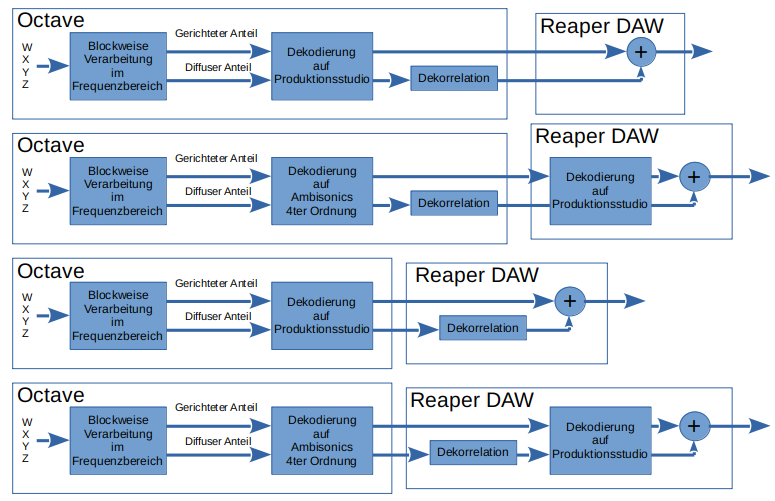
\includegraphics[width=0.9\textwidth]{aufbau/plots/algos.png}
  \label{fig:algos}
  \caption{Flussdiagram Wiedergabe im Produktionsstudio}
\end{figure}

\begin{itemize}
	\item 12 Speaker, Random Phase Decorrelation
	\item 12 Speaker, FDN Decorrelation
	\item T-Design, FDN Decorrelation
	\item T-Design, Widening Plugin
	\item Harpex
	\item Compass
\end{itemize}


\paragraph{Wiedergabesystem}
Als Wiedergabesytem wurde die Lautsprecheranordnung des Produktionsstudios des IEM verwendet.

Bild von Lautsprecheranordnung.

\paragraph{Versuchsinterface}
Um die Antworten der Versuchspersonen auszuwerten wurde die MUSHRA-Anwendung eingesetzt. Diese Anwendung wird über eine \textit{.json}-Datei konfiguriert.

Screenshot von Mushra-Interface.